\documentclass{article}
%\documentclass{statsoc}
\usepackage{fullpage,amsmath,graphicx,sidecap,setspace}
%\usepackage{amsmath,graphicx,sidecap}

%\renewcommand\abstractname{Summary}

\begin{document}

\onehalfspacing

%\begin{titlepage}

 \begin{center}

 \uppercase{  {\Large The statistical uncertainty associated with 
               histograms in the Earth Sciences.}  }

\vspace{.5cm}

 Manuscript accepted for publication in the Journal of Geophysical Research - Solid Earth

 \vspace{.5 cm}

Pieter Vermeesch\\

\vspace{.5 cm}

Department of Geological and Environmental Sciences, Stanford University\\
Braun Hall, room 320-305, 450 Serra Mall\\
Stanford, CA 94305-2115, United States\\
pvermees@pangea.stanford.edu

\vspace{1 cm}

\begin{abstract}
Two  types of  quantitative information  can be  distinguished  in the
Earth  Sciences: categorical  data (e.g.,  mineral type,  fossil name,
...)   and continuous  data (e.g.,  apparent age,  strike,  dip, ...).
Many branches of the Earth Sciences study populations of such data, by
collecting  a   random  sample  and  binning  it   into  a  histogram.
Histograms of categorical  data follow multinomial distributions.  All
possible outcomes of a multinomial distribution with M categories must
plot on a (M-1) simplex  $\Delta_{M-1}$, because they are subject to a
constant-sum  constraint.   Confidence  regions for  such  multinomial
distributions  can   be  computed  using   Bayesian  statistics.   The
conjugate  prior/posterior  to  the  multinomial distribution  is  the
Dirichlet distribution.   A 100(1-$\alpha$)\% confidence  interval for
the unknown multinomial population  given an observed sample histogram
is  a polygon  on $\Delta_{M-1}$  containing 100(1-$\alpha$)\%  of its
Dirichlet posterior.  The projection of this polygon onto the sides of
the simplex yields M confidence intervals for the M bin counts.  These
confidence intervals are ``simultaneous''  in the sense that they form
a  band  completely   containing  the  100(1-$\alpha$)\%  most  likely
multinomial  populations.    As  opposed  to   categorical  variables,
adjacent bins  of histograms  containing continuous variables  are not
mutually   independent.   If  this   ``smoothness''  of   the  unknown
population is  not taken into  account, the Bayesian  confidence bands
described  above will  be  overly conservative.  This  problem can  be
solved by introducing  an {\it ad hoc} prior  of ``smoothing weights''
w=$e^{-sr}$, where r  is the second derivative of  the histogram and s
is a ``smoothing parameter''.\\

\vspace{.5 cm}

%KEYWORDS: Bayes, Dirichlet, histogram, confidence interval, detrital thermochronology
\end{abstract}

 \end{center}

%\end{titlepage}

\section{Introduction} \label{sec:introduction}
Consider  a jar  filled  with  infinitely many  balls  of M  different
colors.   Suppose that  we want  to  estimate the  proportions of  the
colors in the jar by drawing a  sample of N balls from it and counting
the number of times each of  the colors occurs in this sample: {\bf n}
=  \{n$_1$,n$_2$,...n$_M$ $|$ $\sum_{j=1}^{M}$n$_j$  = N\}.   Then our
best guess  (the so-called ``maximum likelihood estimate'')  for the M
proportions  is   {\bf  p}  =   \{p$_1$=n$_1$/N,  p$_2$=n$_2$/N,  ...,
p$_M$=n$_M$/N $|$  $\sum_{j=1}^{M}$p$_j$ =  1\}. Now we  ask ourselves
the question: how confident are we about {\bf p}?  In other words: are
there   any   other  sets   of   proportions   {\bf  p$^{\prime}$}   =
\{p$^{\prime}_1$,    p$^{\prime}_2$,     ...,    p$^{\prime}_M$    $|$
$\sum_{j=1}^{M}$p$^{\prime}_j$  =  1\}  that  could have  yielded  the
observations {\bf n} with reasonable probability?\\

This  simple  statistical  problem  frequently  occurs  in  geological
applications.  Of  course, geologists are not  counting ``balls'', but
things like sediment grains or  faults. Neither are they interested in
``color'' (although  sometimes they do),  but in mineral type,  age or
angle. In  such studies,  the information that  is interpreted  is not
represented by the measurements  themselves, but by estimates of their
probability  distribution, which  are most  often represented  by some
sort of  histogram. When reporting  analytical data, it  is considered
good  scientific practice  to provide  an estimate  of  the associated
statistical uncertainties. This paper presents a method to extend this
practice  to the kind  of point-counting  studies described  above. In
Section \ref{sec:setTheStage}, we will  introduce a number of examples
of histograms  in the Earth Sciences,  as a further  motivation of the
present study.  We will distinguish between two types of histograms. A
first type is  used to represent categorical variables,  such as color
or  mineral type.   Here, we  will also  discuss the  ternary diagram,
which is  a different  way of visualizing  histograms with  only three
bins, that is quite popular  in sedimentary petrography. A second type
of histogram which we will discuss contains continuous, or time series
data.   The prime  examples of  this kind  of histograms  are detrital
thermochronological  grain-age histograms, which  tally the  number of
times  a range  of apparent  grain-ages  occur in  a detrital  sample.
However,  continous histograms need  not necessarily  contain age-data
and we  will see an  alternative example for  which they do  not.  The
fundamental  difference  between   the  aforementioned  two  types  of
histograms  is that the  bins of  categorical histograms  are mutually
independent,   while  adjacent  bins   of  continous   histograms  are
correlated  to  some  degree.    As  a  consequence,  the  method  for
constructing  their  respective  confidence  bands  will  be  somewhat
different.\\

After Section  \ref{sec:setTheStage} has set  the stage, we  can begin
developing  the   statistics  of   the  actual  method   itself.   The
simultaneous confidence bands discussed  in this paper will be derived
according  to the so-called  ``Bayesian'' pradigm,  as opposed  to the
more    traditional     ``frequentist''    paradigm.     In    Section
\ref{sec:independentCI}, these terms will  be explained using a simple
binomial example, which is a degenerate case of the problem this paper
addresses. So by the end of Section \ref{sec:independentCI}, we should
be  in a  good  shape  to compute  simultaneous  confidence bands  for
multinomial   proportions,   which   is   the   subject   of   Section
\ref{sec:simultaneousCI}. Section \ref{sec:frequentist3D} will explain
why  frequentist  confidence intervals  do  not  easily generalize  to
histograms with  more than three  bins. As an alternative,  a Bayesian
method to  construct confidence bands for  categorical histograms will
be   developed  in   Section   \ref{sec:bayes3D}.   Finally,   Section
\ref{sec:bayesSmooth} gives an  {\it ad hoc} way to  modify the method
of  the  preceding   section  so  that  it  takes   into  account  the
autocorrelation      of       continous      histograms.       Section
\ref{sec:examplesRevisited}   revisits   the   examples   of   Section
\ref{sec:setTheStage} and  answers the  questions that were  raised in
it.   Section  \ref{sec:conclusions}  wraps  up the  paper  with  some
summarizing conclusions.

\section{Setting the stage: Examples of histograms in the Earth Sciences} 
\label{sec:setTheStage}
\subsection{Categorical histograms} \label{sec:categorical}

The  framework composition of  sandstones contains  useful information
about  their  provenance,   transport  history  and  post-depositional
evolution, and  is used to  reconstruct the plate-tectonic  setting of
sedimentary  basins (e.g.   Dickinson {\it  et al.},  1983; Dickinson,
1985).    Framework   compositions   are  measured   by   petrographic
point-counting  of thin  sections. The  results are  often  plotted on
ternary diagrams, the most popular  of which is the QFL diagram, which
depicts    quartz,   feldspar,    and    lithic   fragments    (Figure
\ref{fig:QFLa}). As  discussed in Section  \ref{sec:introduction}, one
of  the  questions this  paper  will answer  is  how  to estimate  the
statistical uncertainties  for such point-counting  measurements.  Van
der  Plas  and Tobi  (1965)  discuss  the  construction of  confidence
intervals for  individual point-counting proportions,  for example the
percentage  of quartz  in  a  thin section.   However,  we are  rarely
interested  in  just  a  single  proportion.  This  paper  develops  a
Bayesian  method to  compute {\it  simultaneous} confidence  bands for
categorical histograms.   This method will allow an  estimation of the
likelihood that a  specific sample falls into one  particular field of
tectonic affinity  on the QFL plot (Figure  \ref{fig:QFLa}).  To avoid
confusion, we  should remark  that while this  paper will  discuss the
statistical  uncertainties of  individual  point-counting measurements
(one  sample), it  will  {\it  not} talk  about  the uncertainties  on
populations  of several  measurements.  Whereas  the former  follows a
multinomial distribution, the latter can  take many forms, such as the
logistic normal distribution.   Many interesting issues are associated
with ternary populations, but the  reader is referred to Weltje (2002)
for a discussion of  them.  Figure \ref{fig:QFLa} shows a petrographic
QFL diagram  with tectonic discrimination fields by  Dickinson {\it et
al.}  (1983).   The ''cloud'' of points and  the associated hand-drawn
contour  mark a  detrital population.   For the  discussion of  how to
compute this  contour in a  statistically more rigorous way,  we again
refer to Weltje (2002).  The  present paper will address the following
questions: (1) How different are samples  A and B?  (2) Is it possible
that  samples A and  B belong  to the  contoured population?   (3) How
certain  are we  that sample  C  falls into  the ``transitional  arc''
field?  Could it be that it actually belongs to one of the neighboring
fields?  (4) How does the number of grains affect the precision of our
point-counting results?   Since the  ternary diagram plots  ratios, we
lose information on the actual number of grains counted.  For example,
sample  A represents  200 counts,  while sample  B represents  400 and
there is no way to tell this from Figure \ref{fig:QFLa}.

\begin{figure}[h]
  \centering
  \includegraphics[width=9cm]{QFLa.pdf}
  \caption{Petrographic QFL diagram with tectonic discrimination fields
by Dickinson {\it  et al.} (1983). All samples  except A represent 400
synthetic point-counts. Sample A is based on only 200 counts.}
  \label{fig:QFLa}
\end{figure}

The ternary  diagram is very  popular in sedimentary  petrography, but
when  more than  three  components need  to  be plotted,  we must  use
another  device: the  histogram.  This  is the  case in  heavy mineral
analysis (e.g. Faupl {\it et al.}, 2002), and in clast-counting, which
is a  scaled-up version of petrographic point-counting  (e.g. Yue {\it
et  al.},  2001).   Figure  \ref{fig:heavyminerals1} shows  two  heavy
mineral analyses by  Faupl {\it et al.} (2002).   For each sample, 200
grains were counted.   The basic questions that arise  when doing this
sort of analysis are the same  as for the ternary example: (1) What is
the precision  of the estimated  mineral fractions? (2) How  would the
precision  be affected  by increasing  N, the  total number  of grains
counted? (3)  Are samples ga-229/1  and io-234/1 compatible  with each
other?  Regarding the last question,  it is useful to remark that when
a very large number of grains are counted, it is almost certain that a
statistically significant  difference between two samples  of the same
rock will  be found.  No  two samples collected  on the field  have an
exactly identical composition. As  the number of counts increases, our
power to resolve  even the smallest differences will  increase.  It is
when this  point is reached  that the petrographic composition  of the
sample  has been  properly characterized  and  we can  begin to  study
populations of samples. As a comforting note, we can already tell here
that  the guidelines  of Van  der Plas  and Tobi  (1965)  fulfill this
requirement most of the time.

\begin{figure}[h]
  \centering
  \includegraphics[width=0.5\textwidth]{heavyMinerals1.pdf}
  \caption{
Heavy mineral analysis of two samples from the Peloponnese (Greece) by
Faupl {\it et al.} (2002).  Zr - zircon, Tr - Tourmaline, Rt - Rutile,
Ap -  Apatite, Gt  - Garnet, St  - Staurolite,  Cl - Chloritoid,  Cs -
Chrome spinel.}
  \label{fig:heavyminerals1}
\end{figure}

\subsection{Continuous  histograms (time series)}  \label{sec:continous}

Alternatively,  histograms  can  also  be used  for  continuous  data.
Detrital  thermochronology  tries  to  find  the  provenance  area  of
sedimentary  rocks  and  unravel   its  geologic  history,  by  dating
individual mineral  grains in the  sample (e.g.  Avigad {\it  et al.},
2003;    DeGraaff-Surpless    {\it    et    al.},    2003).     Figure
\ref{fig:Surpless}   shows  three   detrital  zircon   U-Pb  grain-age
distributions  from  the  Methow   Basin,  in  the  southern  Canadian
cordillera (DeGraaff-Surpless  {\it et al.}, 2003).   For each sample,
Figure \ref{fig:Surpless} not only  shows the grain-age histogram, but
also  the continous ``kernel  density estimate''.   Unlike categorical
point-counting  data,  the  grain-ages   that  are  used  in  detrital
thermochronology can have  significant analytical uncertainties.  This
is a second source of  error (the first one being counting statistics)
that is not  taken into account by the  histogram.  The kernel density
estimator is an alternative estimator of probability density that does
take into account measurement  uncertainties.  However, it is not easy
to  estimate  the effect  of  counting  statistics  on kernel  density
estimates.  In  this paper, we will  ignore measurement uncertainties,
and just focus on the effect of counting statistics. We will later see
that in order to get a  better idea of the importance of both factors,
it  is good  practice  to  use histograms  in  conjuction with  kernel
density  estimates.  The reader  is referred  to Silverman  (1986) and
Sircombe and  Hazelton (2004) for  a discussion of the  kernel density
estimator and some issues that  are associated with it.  The questions
this paper  will answer concerning detrital  grain-age histograms are:
(1) What is the uncertainty on the  bin counts? (2) How certain are we
that empty bins actually correspond to missing age fractions?  (3) Are
grain-age   histograms   such   as   the   three   shown   in   Figure
\ref{fig:Surpless}  compatible with  or  significantly different  from
each other?\\

It is  easy to see  that detrital grain-age histograms  represent time
series.  However, continuous histograms are not restricted to the time
dimension.  Figure  \ref{fig:CollettiniHist} shows a  histogram of dip
estimates  for 33  reverse faults  reported by  Collettini  and Sibson
(2001).  Although the units of  this histogram are not time, but angle
(in  degrees), it  still represents  a continous  function,  or ``time
series''.  One of the observations made by Collettini and Sibson about
this histogram  is that it is bimodal,  with one peak at  30$^o$ and a
second  at  50$^o$.  The  simultaneous  Bayesian confidence  intervals
described  in  this   paper  will  tell  us  if   this  bimodality  is
statistically  significant on  for  example a  95\% confidence  level.
Whereas categorical  data follow multinomial  distributions, where the
bins are mutually  independent apart from the fact  that they must sum
to a fixed  number (the sample size), time  series are auto-correlated
to some  degree, and  this must be  taken into account  when computing
confidence intervals.   This paper will assess the  importance of this
problem and propose  a Bayesian solution to it in the  form of an {\it
ad hoc} smoothing prior.

\begin{figure}[h]
  \centering
  \includegraphics[width=12cm]{SurplessMethowSamples.pdf}
  \caption{Three U-Pb grain-age histograms and corresponding kernel density
estimates for  samples of detrital  zircon from the  Cretaceous Methow
basin (DeGraaff-Surpless {\it et al.}, 2003).}
  \label{fig:Surpless}
\end{figure}

\begin{figure}[h]
  \centering
  \includegraphics[width=7cm]{CollettiniHist.pdf}
  \caption{A histogram of 33 reverse fault dip estimates. Although the measurements
are  in  degrees, the  histogram  can  still  be considered  a  ``time
series'',  because  it is  expected  to fit  a  more  or less  smooth,
autocorrelated function.}
  \label{fig:CollettiniHist}
\end{figure}

\clearpage

\section{The definition of a confidence interval}\label{sec:independentCI}

In  this  section,  we  will introduce  some  fundamental  statistical
principles and nomenclature  wich will be needed in  the next section.
Surprisingly enough,  there is no general agreement  in the statistics
community on the  definition of a confidence interval.   There are two
points of  view: the frequentist and  the Bayesian point  of view.  To
explain the difference between these two paradigms, we will consider a
degenerate case of  the problem at hand. Revisiting  the metaphor from
Section \ref{sec:introduction},  we now consider  a jar with  balls of
only two colors,  say black and white.  Drawing N  balls from this jar
as before,  we count the number  n of black balls.   For this binomial
experiment,  the maximum  likelihood  estimate for  the proportion  of
black  balls  in  the  jar  is  p  =  n/N.   How  do  we  construct  a
100(1-$\alpha$)\%   confidence  interval   for   this  estimate?    An
approximate solution to this problem is given by Van der Plas and Tobi
(1965), but both  the frequentist and the Bayesian  methods which will
be discussed now are exact.

\subsection{The frequentist approach}\label{sec:frequentist2D}

According  to  the  ``frequentist'',   a  confidence  interval  for  a
parameter $\theta$  {\it ``consists precisely  of all those  values of
$\theta_0$ for which the null hypothesis H$_0$: $\theta$=$\theta_0$ is
accepted''} (Rice, 1995).  For example, we saw earlier that histograms
represent the  outcome of  a multinomial experiment.   The probability
distribution of each of the bin  counts of a histogram is the marginal
of  a multinomial  distribution, which  is the  binomial distribution.
Consider  a bin  containing  n  out of  N  measurements.  The  maximum
likelihood   estimate   for  the   binomial   parameter   p  then   is
$\hat{p}_{mle} = n/N$.  Now  consider the null hypothesis $H_0: p=p_o$
versus  the alternative $H_a:  p \neq  p_o$.  $H_0$  is accepted  on a
100(1-$\alpha$)\% confidence level iff:
\begin{equation}
  \label{eq:hypothesis}
\sum_{i=n}^N  \binom{N}{i} p_o^i  p_o^{N-i} < 
\frac{\alpha}{2} <
\sum_{i=0}^n  \binom{N}{i} p_o^i  p_o^{N-i} 
\end{equation}
Now,  according to  the  definition, a  two-sided confidence  interval
contains  all those  values for  $p_o$ which  pass the  test  given by
Equation \ref{eq:hypothesis}.  The solution  can be found by numerical
iteration  and/or  interpolation  (Clopper  and  Pearson,  1934).   An
example   for    N=50,   n=20    and   $\alpha$=0.1   is    given   in
Figure~\ref{fig:frequentist2D}.

\begin{figure}[h]
  \centering
  \includegraphics[width=8cm]{2.pdf}
  \caption{90\% frequentist confidence bounds on p for n=20,N=50. The
  step-functions represent  the cumulative binomial  distribution with
  parameters (N,$\b{p}$) and  (N,$\bar{p}$), respectively.  $\b{p}$ is
  the largest  value for p for which  20 out of 50  counts would occur
  more than 5\%  of the time. Likewise, $\bar{p}$  is the lowest value
  for p  that would yield the  observed ratio of 20/50  with more than
  5\% probability.}
  \label{fig:frequentist2D}
\end{figure}

It can be shown (e.g. Blyth, 1986), that Equation \ref{eq:hypothesis}
is mathematically equivalent to:
\begin{equation}
  \label{eq:blythe}
  \b{p}  = B(1-\frac{\alpha}{2},n+1,N-n)<p<B(\frac{\alpha}{2},n,N-n+1)
  = \bar{p}
\end{equation}
Where  $B(\alpha,a,b)$ is  the 100$\alpha$  percentile of  the $\beta$
distribution with parameters a and b:
\begin{equation}
  \label{eq:beta}
  \beta(a,b)=\frac{\Gamma(a+b)}{\Gamma(a)\Gamma(b)}p^{a-1}(1-p)^{b-1}
\end{equation}
where $\Gamma$(x) is  the gamma function, which can  be considered the
continuous version of the factorial  operator. For example, if x is an
integer, then $\Gamma$(x+1)=x!. Likewise, the $\beta$ distribution can
be  thought  of  as  being   a  continuous  version  of  the  binomial
distribution. Notice  that for  n=0 and n=N,  Equation \ref{eq:blythe}
breaks down. Instead, the following expressions should be used:
\begin{eqnarray}
  \label{eq:blythespecial}
   \b{p} = &0 < p < 1-\alpha^{1/N} = \bar{p}   &\mbox{ if n=0, or}\\
   \b{p} = &(1-\alpha)^{1/N} < p < 1 = \bar{p} &\mbox{ if n=N}
\end{eqnarray}

\subsection{The Bayesian approach}\label{sec:bayes2D}

For  a  ``Bayesian'',  a  100(1  -  $\alpha$)\%  confidence  (or  {\it
credibility}) interval  for a parameter $\theta$ given  some data {\bf
x} is an interval for $\theta$  that covers 100(1 - $\alpha$)\% of its
{\it posterior  distribution} P($\theta | {\bf x})$,  where the latter
is given by:
\begin{equation}
  \label{eq:4}
  P(\theta | {\bf x}) \propto P({\bf x}|\theta)P(\theta)
\end{equation}
with  P($\theta$) a {\it  prior distribution}  on $\theta$  and P({\bf
x}$|\theta$)  the {\it  likelihood  function} of  the  data given  the
parameter.   The subjectivity  of the  Bayesian approach  lies  in the
choice  of  the prior  distribution.   A  uniform distribution  (``flat
prior'') is often  taken if no prior information exists  as to what the
value of $\theta$  should be.  However, whether or not  this is a good
{\it  non-informative}   prior  has  been   challenged.   The  uniform
distribution does not yield posterior distributions that are invariant
under  reparameterization  (Jeffreys,  1946).   We will  soon  see  an
example  of an  alternative  prior distribution  that  does have  this
invariance.\\

We now return to the  problem of independent credibility intervals for
multinomial proportions. Again, we consider a bin with n counts out of
N and  want to construct a 100(1-$\alpha$)\%  credibility interval for
p=n/N.  The  likelihood function  is binomial: $P(n|p)  = \binom{N}{n}
p^n p^{N-n}$.  If we take a flat prior for P(p), then the posterior is
a $\beta(n+1,N-n+1)$ distribution (Bayes, 1763):
\begin{equation}
  \label{eq:betabayes}
  P(q<p<r | n) = \frac{\Gamma(N+2)}{\Gamma(n+1)\Gamma(N-n+1)}
                 \int_q^rp^{n}(1-p)^{N-n}dp
\end{equation}
Therefore:
\begin{equation}
  \label{eq:bayes2D}
 \b{p} = B(1-\frac{\alpha}{2},n+1,N-n+1)<p<B(\frac{\alpha}{2},n+1,N-n+1) = \bar{p}
\end{equation}
Notice   the  similarities   between  Equations   \ref{eq:blythe}  and
\ref{eq:bayes2D}.   However, as  opposed to  the  frequentist Equation
\ref{eq:blythe},  the Bayesian  Equation  \ref{eq:betabayes} does  not
require a special case for n=0 and n=N. The $\beta$ distribution is an
example of  a {\it  conjugate prior}.   This means that  if we  take a
$\beta$-distributed prior, and  a binomial sampling distribution, then
the  posterior will  also have  a $\beta$  distribution.   The uniform
distribution is a  special case of the $\beta$  distribution for a=b=1
(i.e.    $\beta(1,1)$).   $\beta$($\frac{1}{2}$,$\frac{1}{2}$)   is  a
noninformative  prior   ({\it  Jeffreys'  prior})   for  the  binomial
distribution that  is invariant under  reparameterization (e.g.  Gill,
2002,    p.124).    The    posterior    distribution   then    becomes
$\beta$(n+$\frac{1}{2}$,N-n+$\frac{1}{2}$).   Taking the  same example
as   for   Section    \ref{sec:frequentist2D}   (i.e.    n=20,   N=50,
$\alpha$=0.1), Figure \ref{fig:Bayesian2D}  shows a two-sided Bayesian
credibility interval for p.
\begin{figure}[here]
  \centering
  \includegraphics[width=8cm]{3.pdf}
  \caption{90\% Bayesian credibility bounds on p for n=20,N=50. The 
curve  represents the  cumulative $\beta$  distribution  function with
parameters n+1 and N-n+1, using a flat prior. The credibility interval
[  $\b{p} <$ p  $< \bar{p}$  ] is  a (symmetric)  interval for  p that
covers 90\% of the area under this posterior distribution.}
  \label{fig:Bayesian2D}
\end{figure}

\section{Simultaneous confidence intervals for multinomial proportions}
\label{sec:simultaneousCI}

As was shown in Section \ref{sec:independentCI}, it is relatively easy
to construct {\it independent} confidence  intervals for each of the M
bin counts  $n_m$ ($1 \leq m \leq M$) that make up  a histogram, both
under the frequentist  and the Bayesian paradigm. However,  we need to
be  more ambitious  than that.   In order  to be  able to  compare two
samples and test if they are significantly different, we would like to
construct  {\it simultaneous} confidence  intervals for  all of  the M
histogram  bins. Like we  did for  the binomial  case in  the previous
section,  we will  again discuss  first the  frequentist and  then the
Bayesian solution to  this problem. It will soon  become clear why the
Bayesian method is more appropriate for our purpose.

\subsection{Frequentist Confidence Regions} \label{sec:frequentist3D}

As  discussed before,  histograms are  representations  of multinomial
distributions.   Suppose we  have N  numbers  (``balls''), distributed
over M bins (``colors''),  corresponding to M multinomial proportions.
The   bin   counts   ($n_1,...,n_M$)   must  fulfill   the   condition
$\sum_{m=1}^{M}n_m$=N.     Therefore,    all   possible    multinomial
distributions  must fall  on  an {\it  M-simplex} $\Delta_{M-1}$.   An
example  of a  3-simplex (which  just  is another  word for  ``ternary
diagram'') is shown on Figure \ref{fig:simplex}.  Consider a histogram
with    M    bins,   representing    a    sample    of   N    numbers:
$X_N=\{x_1,...,x_N\}$.   This histogram  corresponds to  one  point on
$\Delta_{M-1}$, the {\it maximum likelihood estimate} (mle) of the bin
counts.    Under  the  frequentist   paradigm,  outlined   in  Section
\ref{sec:frequentist2D},  a  100(1-$\alpha$)\%  confidence  region  on
$\Delta_{M-1}$  consists of all  those probability  vectors {\bf  p} =
($p_1,...,  p_M~|~\sum_{m=1}^M p_m=1$) which  are capable  of yielding
observations  as   extreme  as   {\bf  n}  =   ($n_1,  ...,   n_M  ~|~
\sum_{m=1}^Mn_m = N$) with at least 100(1-$\alpha$)\% probability.\\

In order  to find  this region,  a grid of  possible {\bf  p}$^{kl}$ =
($p_1^{kl},...  ,p_M^{kl} ~|~ \sum_{m=1}^Mp_m^{kl} = 1$) is evaluated.
For each of  these ``test-populations'' (for example the  black dot on
Figure  \ref{fig:convHull}) a  large number  of  synthetic ``samples''
(the white  dots on Figure  \ref{fig:ternFreqBoot}) of N  numbers were
generated,  following an  algorithm  given in  Appendix  A.  Next,  we
construct  the  100$\alpha$\% {\it  convex  hull}  of these  synthetic
samples.  This  is a  polygon containing 100$\alpha$\%  (the so-called
``hull percentile'') of them.  We  test to see if {\bf p}$^{mle}$ (the
black  square on  Figure \ref{fig:convHull})  falls within  the convex
hull of {\bf  p}$^{kl}$. If this is not the  case, then {\bf p}$^{kl}$
falls   outside   the   100$\alpha$\%   confidence  region   of   {\bf
p}$^{mle}$. This procedure is repeated  for the entire grid (k=1...K ,
l=1...L).  On Figure \ref{fig:ternFreqBoot}, the contour line contains
all  those  grid  points for  which  the  mle  falls within  their  95
percentile hull.\\

Figures \ref{fig:convHull} and \ref{fig:ternFreqBoot} just serve as an
illustration  of  the  frequentist  paradigm on  $\Delta_2$.   A  more
efficient way to compute approximate frequentist confidence regions on
the ternary diagram is  described by Weltje (2002, p.246).  Projecting
the frequentist confidence  region onto the axes of  the simplex would
not represent that region, but the smallest polygon circumscribing it.
Therefore,  it   is  not   possible  to  accurately   ``translate''  a
frequentist contour plot to error  bars on a histogram, which makes it
impossible  to  easily  visualize  the  frequentist  uncertainties  of
histograms with more than three bins. The Bayesian credibility regions
discussed next solve this problem.

\begin{figure}[here]
  \centering
  \label{fig:convHull}
  \includegraphics[width=8cm]{4.pdf}
  \caption{
To  test  if  the  trinomial  distribution marked  by  the  black  dot
(p$_1$=1/2,p$_2$=1/6,p$_3$=1/3) belongs to  the 95\% confidence region
of   the   trinomial   experiment   marked   by   the   black   square
(n$_1$=5,n$_2$=10,n$_3$=15),  a  large   number  (1000)  of  trinomial
samples of  N=30 numbers was  generated from this  distribution.  They
are  represented  by  the   open  circles.   The  black  contour  line
represents the 95\% convex hull.  Since the black square does not fall
within  this hull,  the black  dot falls  outside the  95\% confidence
region of the trinomial experiment.}
\end{figure}

\begin{figure}[here]
  \centering
  \label{fig:ternFreqBoot}
  \includegraphics[width=8cm]{5.pdf}
  \caption{
The black  dots represent the  maximum likelihood estimates  (mle) for
two    trinomial   experiments    (\{n$_1$=5,n$_2$=10,n$_3$=15\}   and
\{n$_1$=15,n$_2$=15,n$_3$=0\}).   The  black  contours  represent  the
frequentist confidence  regions, obtained by  repeating the experiment
shown in Figure \ref{fig:convHull} on  a 1250 point grid.  For each of
the  grid points, B=200  trinomial samples  were generated.   The gray
lines outline  the Bayesian credibility regions (using  a flat prior).
The agreement between the two methods is surprisingly good.}
\end{figure}

%\clearpage

\subsection{Bayesian Credibility Regions}
\label{sec:bayes3D}

It  is  relatively easy  to  generalize  the  methodology outlined  in
Section \ref{sec:bayes2D} from a  binomial to a multinomial situation.
Recall  that the  conjugate prior  to a  binomial distribution  is the
$\beta$-distribution.    The   conjugate   prior  to   a   multinomial
distribution is the {\it Dirichlet distribution}:

\begin{equation}
  \label{eq:dirichlet}
  D_{\bf a}(p_1,...,p_M)=
  \frac{\Gamma(\sum_{i=1}^{i=M}{a_i})}{\prod_{i=1}^{i=M}\Gamma(a_i)}
  \prod_{i=1}^{i=M}p_i^{a_i-1}
\end{equation}

The  multinomial  uniform  distribution  is  a  special  case  of  the
Dirichlet distribution with all a$_i$=1.  If  {\bf n} is a vector of M
bin counts, then the posterior distribution under such a flat prior is
D$_{{\bf  n}+1}$($p_1$,...,$p_M$).   The choice  of  a  prior that  is
truely non-informative and  invariant under reparameterization is more
controversial  for   the  Dirichlet  than  it  was   for  the  $\beta$
distribution.   Jeffreys  suggested   taking  a$_i$=1/2,  while  Perks
recommended using a$_i$=1/M ($\forall$ i=1...M) (Good, 1965).  Similar
to  the   binomial  case  (Section   \ref{sec:bayes2D}),  simultaneous
Bayesian  credibility  bands  for  the  multinomial  distribution  are
intervals that cover 100(1-$\alpha$)\% of the area under the posterior
distribution.   A few examples  of Dirichlet  posteriors are  shown on
Figure \ref{ternAnDir}.  As opposed to the $\beta$ distribution, there
are no  tables of the  percentiles of the Dirichlet  distribution.  In
order to integrate this  multi-dimensional function ourselves, we have
to numerically sample  from it, as described by  Devroye (1986) and in
Appendix B.\\

Thus,  a collection  of B  ``sample histograms''  can  be constructed,
representing  B  samples  from  the posterior  Dirichlet  distribution
(Figure \ref{terNumDir}).   All these histograms  correspond to points
on $\Delta_{M-1}$.   Asymptotically, {\it independent} 100$(\alpha/2)$
and 100($1-\alpha/2$)  percentiles for the  replicates of each  of the
histogram  bin counts  will  converge to  the independent  credibility
intervals of Equation \ref{eq:bayes2D}.   However, it is also possible
to obtain  {\it simultaneous} credibility bands.  The  Bayesian way of
doing this is to find M credibility intervals that define a polygon on
$\Delta_{M-1}$   containing   100(1-$\alpha$)\%   of   the   posterior
distribution  (Figures  \ref{fig:simplex}  and \ref{terNumDir}).   The
algorithm for  finding this polygon  is given in Appendix  B.  Figures
\ref{fig:compPriors}   and  \ref{fig:dirHist}   show  the   effect  of
different priors  on the posterior distribution  and its corresponding
credibility polygon.\\

This Bayesian  method yields non-zero credibility  intervals, even for
empty  bins.  It  works  for  histograms but  not  for kernel  density
estimates,  which  are  continuous  functions that  cannot  be  easily
represented  on a simplex.   As histograms  traditionally do  not take
into account measurement uncertainties, the Bayesian credibility bands
only reflect the uncertainties induced by the counting statistics, and
not those caused by analytical  imprecision. A final remark to be made
is  that, strictly  speaking,  the way  we  have defined  simultaneous
Bayesian  credibility  regions is  only  exact  for {\it  categorical}
histograms,   such  as  those   obtained  by   point-counting  mineral
assemblages.   However, if  the  histogram represents  a time  series,
which is the case in detrital thermochronology, it will have some {\it
smoothness} to it.   This effect will not be  captured by the Bayesian
credibility  regions  discussed   before.   The  categorical  Bayesian
credibility bands can  be overly conservative if applied  to such {\it
autocorrelated} data.   The next section  of the paper  discusses this
issue.

\begin{figure}[here]
  \centering
  \label{fig:simplex}
  \includegraphics[width=8cm]{6.pdf}
  \caption{
All possible outcomes  of a trinomial experiment, for  example a 3-bin
histogram of  N measurements x$_i$  plot on a 3-simplex.   The maximum
likelihood  estimate  for  the  multinomial proportions  is  given  by
p$_m^{mle}$=(\#$x_i$s in m$^{{th}}$bin)/N  (m=1,2 and 3).  The maximum
likelihood etimate (mle) is represented by a black dot.  The posterior
distribution of the unknown parameters p$_1$, p$_2$ and p$_3$ is given
by a  Dirichlet distribution.  To  find simultaneous 100(1-$\alpha$)\%
confidence bounds for  these parameters, we need to  find a polygon on
the   simplex  that  contains   100(1-$\alpha$)\%  of   the  posterior
distribution.}
\end{figure}

\begin{figure}[here]
  \centering
  \includegraphics[width=0.32\textwidth]{7a.pdf}
  \includegraphics[width=0.32\textwidth]{7b.pdf}
  \includegraphics[width=0.32\textwidth]{7c.pdf}
  \caption{
Analytical contours  for different posterior  Dirichlet distributions.
The  parameters  are,  from  left  to right:  (1,2,3),  (5,10,15)  and
(0,0,5).   Comparison  of  the  leftmost  two figures  shows  how  the
posterior Dirichlet distribution is more tightly constrained when more
data are  used. The rightmost plot  shows how, even when  two bins are
empty, meaningful confidence intervals can be computed.}
  \label{ternAnDir}
\end{figure}

\begin{figure}[here]
  \centering
  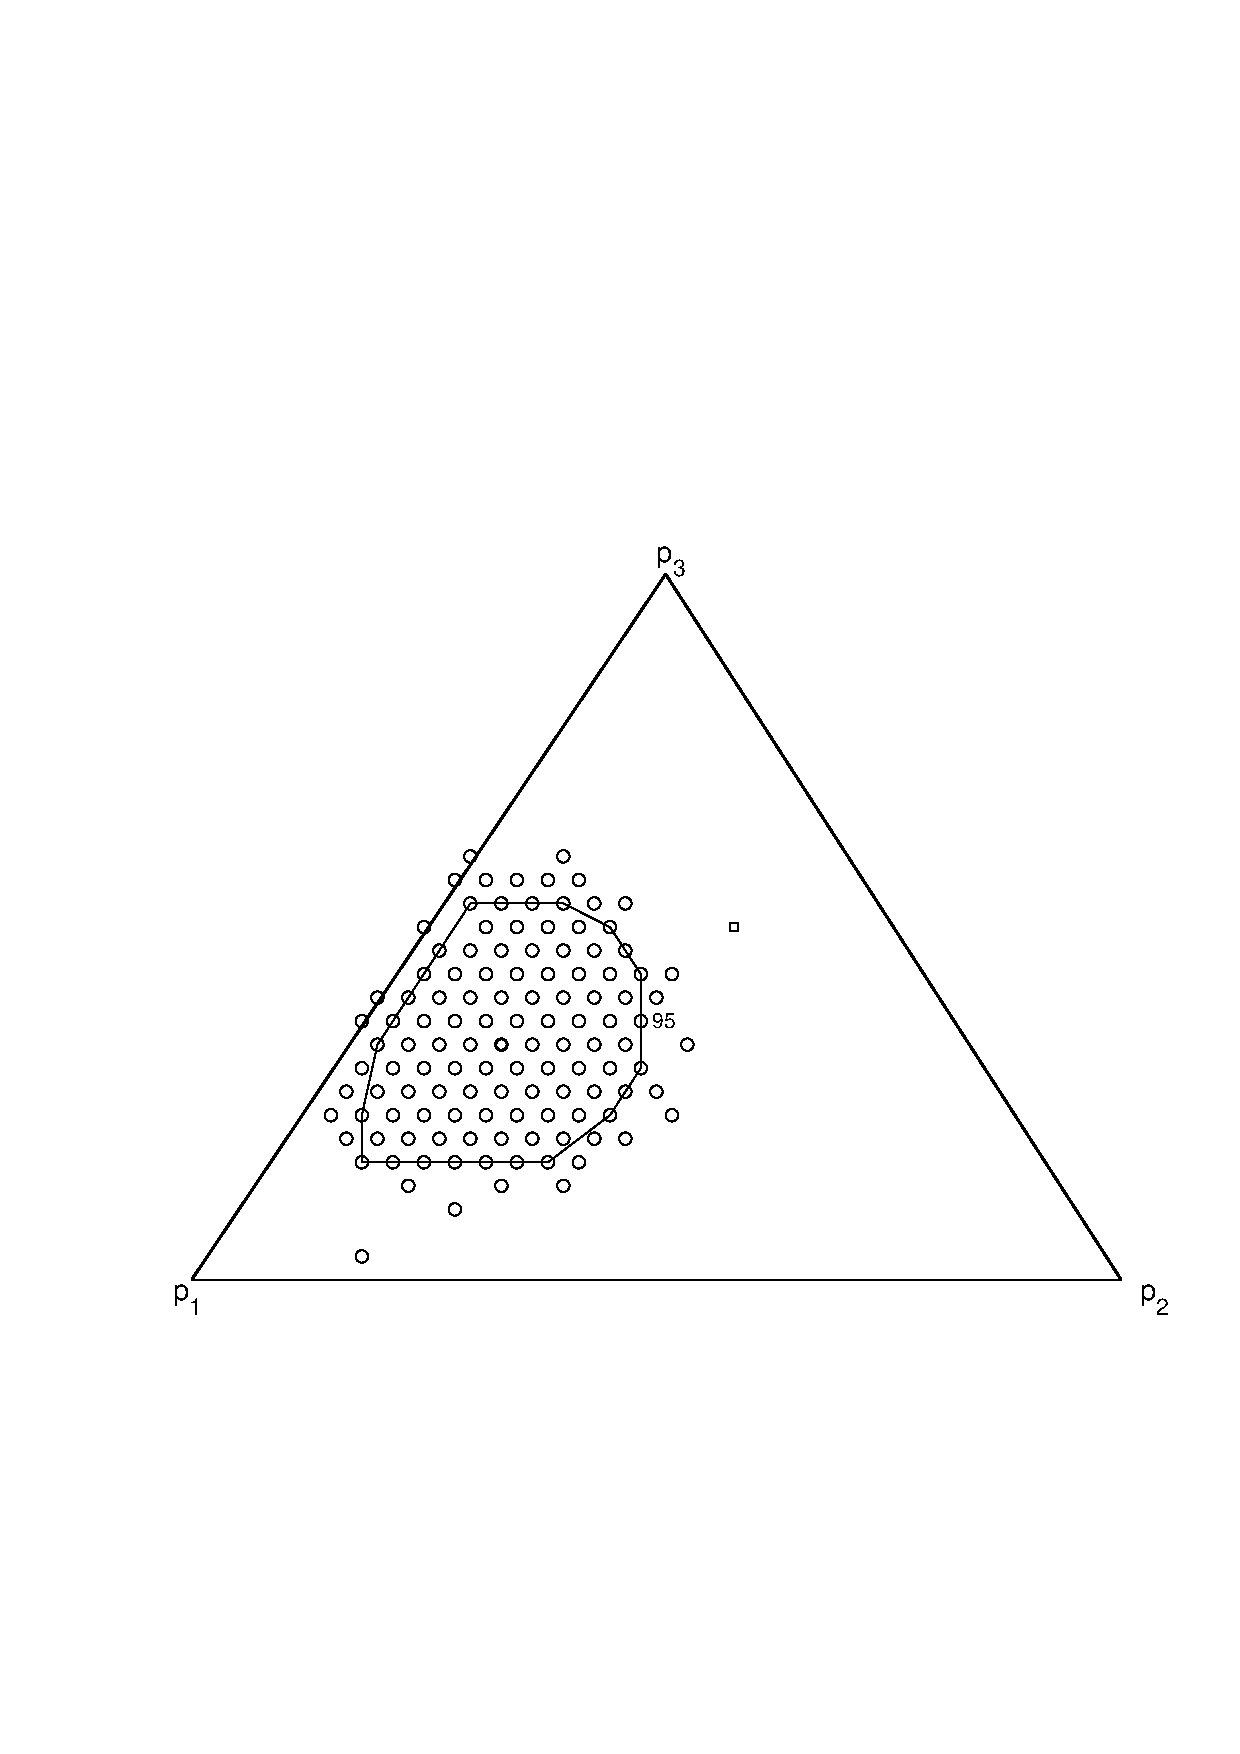
\includegraphics[width=8cm]{8.pdf}
  \caption{
The  area  under  posterior  distributions  such as  those  in  Figure
\ref{ternAnDir} can  be numerically  integrated.  The white  dot shows
the maximum likelihood trinomial  distribution for a particular sample
(n$_1$=5, n$_2$=10,  n$_3$=15).  The black dots  represent 1000 random
samples from the Dirichlet posterior distribution D$_{6,11,16}$ on the
3-simplex.  The polygon contains  95\% of these points. The projection
of this polygon onto the  three parameter axes yields the simultaneous
Bayesian credibility intervals.}
  \label{terNumDir}
\end{figure}

\begin{figure}[here]
  \centering
  \label{fig:compPriors}
  \includegraphics[width=8cm]{9.pdf}
  \caption{
The black dots on this 3-simplex represent sample bin counts (5,10,15)
and (15,15,0).   The solid  black polygons represent  their respective
simultaneous  95\% Bayesian  credibility polygons  with  uniform prior
D$_{1,1,1}$,   while   for   the   dashed   polygons,   Perks'   prior
D$_{\frac{1}{3},\frac{1}{3},\frac{1}{3}}$ was used.}
\end{figure}

\begin{figure}[here]
  \centering
  \includegraphics[width=10cm]{syntheticHist.pdf}
  \caption{
The white  histograms represent a synthetic  population of categorical
variables, the  black histogram  a sample of  50 items from  it.  Note
that the  sample completely missed  the 5$^{th}$ population  bin.  The
gray band  covers 95\%  of the posterior  distribution for (a)  a flat
(uniform)  prior,  and  (b)  Perks'  prior.   Both  credibility  bands
correctly contain the original population.}
  \label{fig:dirHist}
\end{figure}

\clearpage

\subsection{Bayesian credibility bands for smooth histograms} 
\label{sec:bayesSmooth}

Strictly speaking,  Bayesian credibility bands are  only applicable to
non-smooth or  categorical data (Section  \ref{sec:bayes3D}).  In this
section, we will  discuss the importance of this problem  and a way to
solve it.  We can express the  {\it roughness} r of a time series g(t)
as a function {\it f} of its second derivative:

\begin{equation}
  \label{eq:contRoughness}
  r(g(t))  = \mbox{\Large{\it f}} \left(  \int\left(\frac{d^2 g(t)}{dt^2}\right)^2dt
  \right)
\end{equation}
For example, for the discrete case of a histogram with three bins {\bf
n}=(n$_1$,n$_2$,n$_3$), we could write:
\begin{equation}
  \label{eq:discSmoothness}
  r({\bf n}) = \left(n_1-2n_2+n_3\right)^2
\end{equation}
We now define the {\it smoothness weight} w as:
\begin{equation}
  \label{eq:smoothness}
  w = e^{-sr}
\end{equation}
where    s    is    the    {\it    smoothing    parameter}.     Figure
\ref{fig:ternDirWeights}  shows the  trinomial  smoothing weights  for
different   values  of   s  (for   fixed   N=n$_1$+n$_2$+n$_3$).   The
distribution of the weights can  be used to {\it filter} the posterior
distribution, thereby in effect  serving as a {\it prior distribution}
(a ``smoothing  prior''). The  algorithmic details for  this procedure
are given in Appendix C.

\begin{figure}[here]
  \centering
  \includegraphics[width=0.32\textwidth]{11c.pdf}
  \includegraphics[width=0.32\textwidth]{11b.pdf}
  \includegraphics[width=0.32\textwidth]{11a.pdf}
  \caption{
Contoured  smoothing priors for  different smoothing  parameters, with
N=n$_1$+n$_2$+n$_3$=10.   From left  to  right: s=0  (no smoothing)  ,
s=0.1  (weak smoothing),  and s=1  (strong smoothing).   The strongest
weights are  located along the p$_2$=n$_2$/N=1/3  line, which connects
all possible histograms with zero second derivative.}
  \label{fig:ternDirWeights}
\end{figure}

\begin{figure}[here]
  \centering
  \includegraphics[width=8cm]{12.pdf}
  \caption{Smoothed version of Figure \ref{terNumDir}, using
s=0.1 }
  \label{fig:smoothTernDir}
\end{figure}

Figure  \ref{fig:smoothTernDir}  shows the  results  of  this kind  of
posterior  filtering for  a trinomial  distribution on  $\Delta_2$.  A
logical extension  of this  method from  three to M  bins would  be to
replace Equation \ref{eq:discSmoothness} by:

\begin{equation}
r({\bf n}) = \sum_{m=2}^{M-1}\left(n_{m-1} - 2n_m + n_{m+1}\right)^2
\label{eq:discSmoothnessMgt3}
\end{equation}

By generating  samples from the posterior  distribution, and accepting
or rejecting  them based on  the smoothing weights given  by Equations
\ref{eq:smoothness}  and \ref{eq:discSmoothnessMgt3},  B  samples from
the  smoothed posterior  could be  obtained.  However,  the  amount of
computation  time that would  be required  for this  process increases
exponentially with M.  The  ``sliding window'' approach explained next
does a similar job in  linear time.  The roughness penalty embodied by
Equation  \ref{eq:smoothness} depends on  the second  derivative only.
This means that we only consider the influence of immediately adjacent
bins  on  each other.   For  example,  the  m$^{th}$ bin  is  directly
correlated with the (m-1)$^{th}$ bin and the (m+1)$^{th}$ bin, but not
with the (m-2)$^{th}$ bin and the (m+2)$^{th}$ bin.  This warrants the
use of a  three bin wide ``sliding window'',  that recursively smooths
the posterior distribution from the  left to the right (or vice versa)
one bin  at a time. The details  of this method are  given in Appendix
C.\\

Figures  \ref{fig:sineSmooth} and  \ref{fig:triangleseries} illustrate
the results  of the sliding  window procedure on a  synthetic dataset.
These figures demonstrate how using  a smoothing prior filters out the
roughest ``spikes''  from the posterior  sample set. It is  such often
small  minority of  outliers  that makes  the unsmoothed,  categorical
confidence  bands of Section  \ref{sec:bayesSmooth} too  wide, meaning
too conservative, for continuous histograms. An example of the sliding
window   approach    on   real    data   is   deferred    to   Section
\ref{sec:continuousRevisited}, where we will also discuss which values
for the  smoothing parameter s to  choose, and why the  rather {\it ad
hoc}  nature of  the smoothing  method  discussed in  this section  is
probably not a big issue after all.

\begin{figure}[here]
  \centering 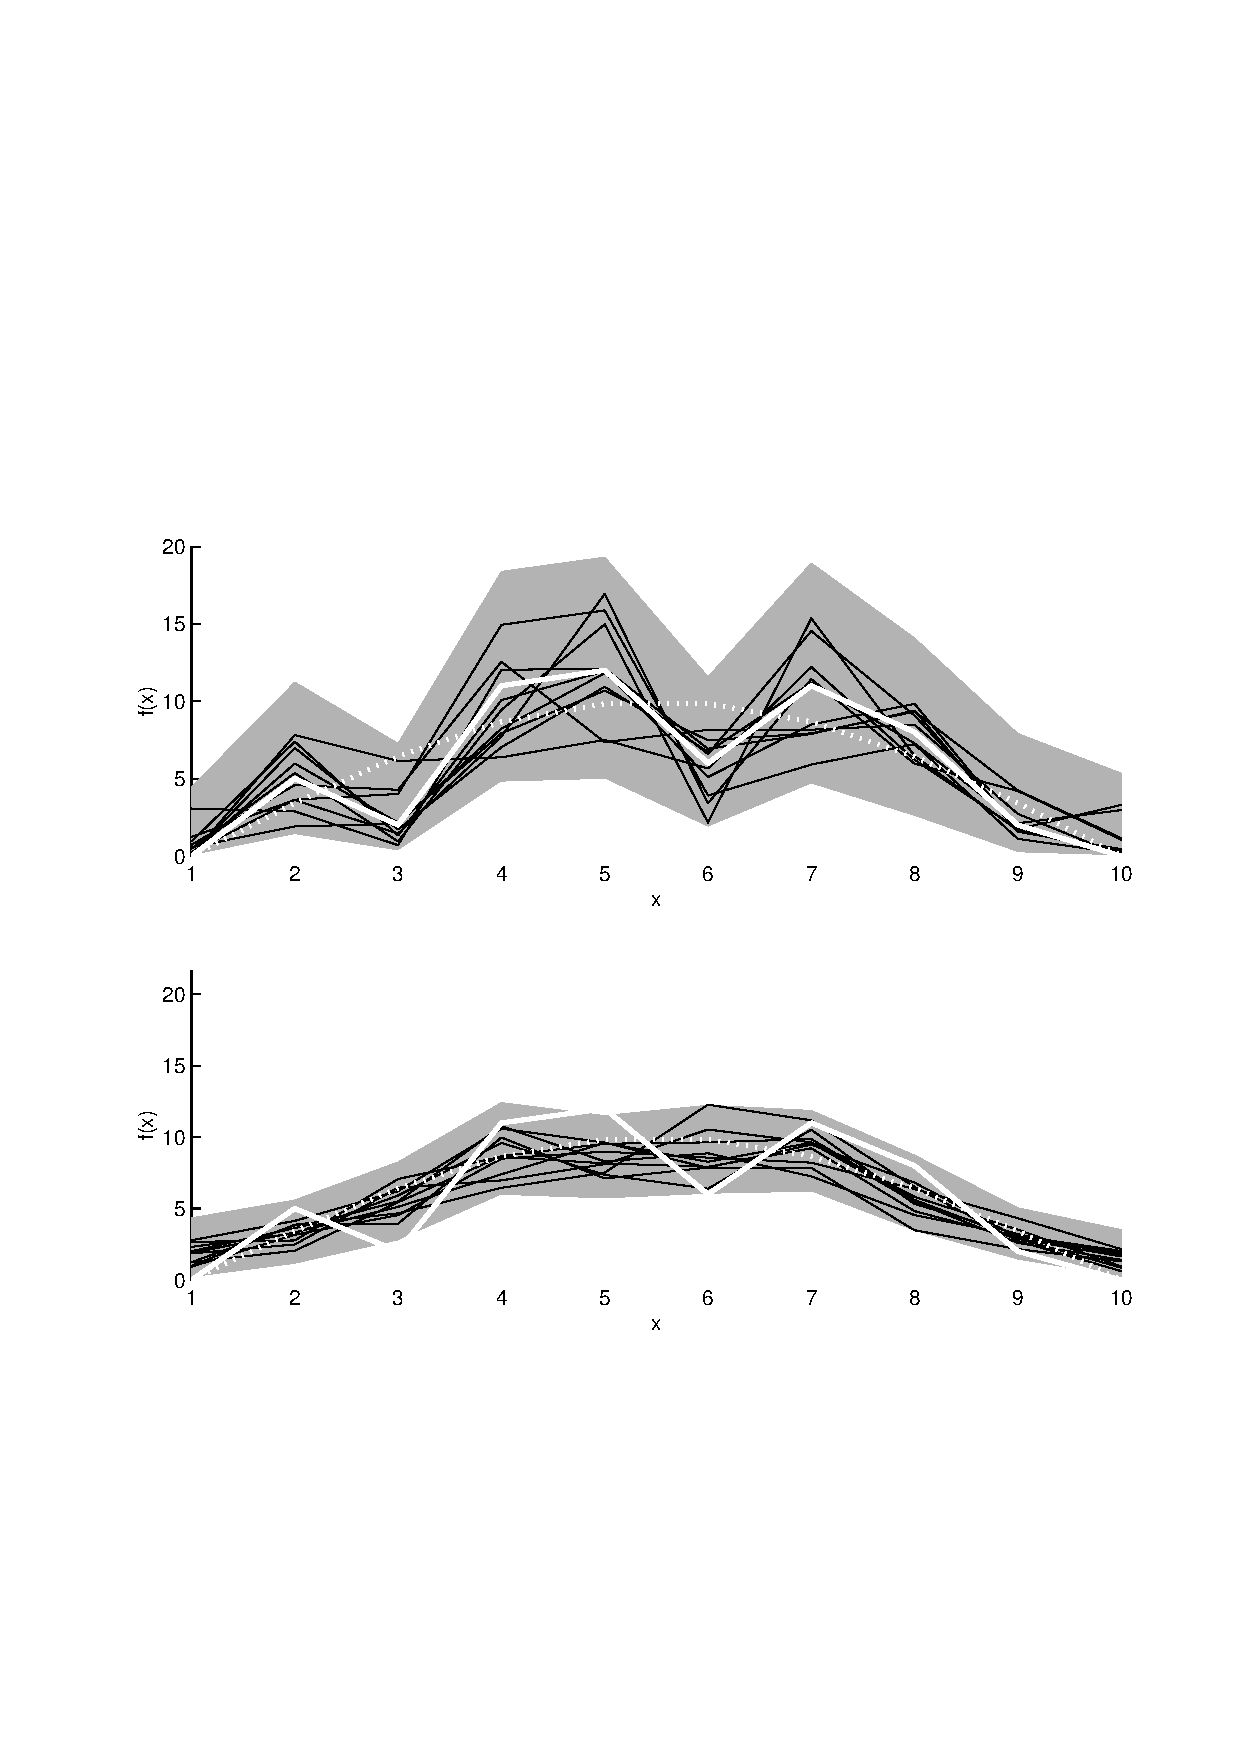
\includegraphics[width=9cm]{14.pdf}
  \caption{
The dashed white lines show  the histograms --or rather {\it frequency
polygons} (Scott, 1992)-- of a smooth population (sine function).  The
solid  white lines  show  the frequency  polygons  of a  sample of  57
numbers that were randomly drawn from this population.  The gray areas
mark the simultaneous 95\% credibility bands, obtained by the Bayesian
method and based  on 500 samples from the  posterior distribution.  10
of these  samples are shown in  black to illustrate the  effect of the
smoothing prior.   The non-smoothed  Bayesian credibility band  (a) is
about twice as wide as the smoothed credibility band (b).}
  \label{fig:sineSmooth}
\end{figure}

\begin{figure}[here]
  \centering
  \includegraphics[width=\textwidth]{14a+b.pdf}
  \caption{Trinomial ``slices'' through the unsmoothed (top) and smoothed 
(bottom) posteriors of Figure \ref{fig:sineSmooth}.
}
  \label{fig:triangleseries}
\end{figure}

\clearpage 

\section{Case studies} \label{sec:examplesRevisited}

\subsection{Categorical histograms} \label{sec:categoricalRevisited}

We  first  return  to  the  example previously  discussed  in  Section
\ref{sec:categorical} and illustrated by Figure \ref{fig:QFLa}. Figure
\ref{fig:QFLb}  shows  the   simultaneous  95\%  Bayesian  credibility
regions  for samples  A-D  on the  ternary  QFL diagram  in their  now
familiar  polygonal  form.   The  difference between  the  credibility
regions of samples A and B  clearly stands out. Recall that 400 points
were counted for sample  B, as opposed to only 200 for  sample A. As a
result, the uncertainty polygon of A is substantially larger than that
of B.  It  is quite possible that  A and B were sampled  from the same
distribution. Whereas it  very unlikely that sample B  could have been
derived from  the population outlined by the  contour, this conclusion
cannot be made for sample A.  A similar situation exists for sample C.
This  sample plots  into the  ``transitional  arc'' field  of the  QFL
diagram,  but its  95\%  uncertainty region  partly  falls inside  the
``undissected arc'' and ``recycled  orogen'' fields.  Although we have
not  done so,  it would  even be  possible to  compute  the respective
probabilities  for  the  three  fields,  by  counting  the  number  of
numerical Bayesian replicates that  fall into them.  Finally, sample D
contains only one percent  (4/400) of quartz.  Its uncertainty hexagon
is  highly asymmetric  but falls  entirely inside  the simplex,  as it
should.\\

\begin{figure}[h]
  \centering
  \includegraphics[width=9cm]{QFLb.pdf}
  \caption{The QFL diagram of Figure \ref{fig:QFLa}, with
95\% credibility  regions for  samples A-D.  The  hexagon of  sample A
(200  point-counts) is  markedly larger  than  that of  sample B  (400
point-counts). Sample  C most  likely falls inside  the ``transitional
arc'' field, but there is more  than 5\% likelihood that it belongs to
either the ``undissected arc'' or ``recycled orogen'' field.}
  \label{fig:QFLb}
\end{figure}

We now proceed to the multinomial example of heavy mineral analyses by
Faupl {\it  et al.} (2002). Figure  \ref{fig:heavyminerals2} shows the
95\% credibility  intervals for  the eight heavy  mineral proportions,
using   Jeffreys'   prior.   When   200   grains   are  counted,   the
percentage-error  is  between  2  (staurolite in  ga-229/1)  and  20\%
(garnet  in io-234/1)  (Figure \ref{fig:heavyminerals2}.a).   There is
less  than 5\%  probability  that the  heavy  mineral distribution  of
sample io-234/1 is compatible with that of sample ga-229/1 because the
observed  apatite and garnet  fractions of  io-234/1 fall  outside the
simultaneous 95\%  credibility band of ga-229/1. Likewise,  it is less
than  5\% likely  that  sample ga-229/1  is  compatible with  io-234/1
because the  apatite and garnet  fractions of the former  fall outside
the confidence  bands of the  latter. The statement that  ga-229/1 and
io-234/1 are mutually compatible is true with less than 2.5\%, and not
5\% probability, because it  involves two simultaneous tests.  This is
a  consequence of  the so-called  Bonferroni inequality  (Rice, 1995).
The  Bonferroni   rule  is   on  the  conservative   side,  especially
considering the fact  that the two tests are  not entirely independent
from each other.  Figure  \ref{fig:heavyminerals2}.b shows that if the
percentages reported  by Faupl  {\it et al.}   had been the  result of
counting 1000 instead of  200 grains, the percentage-errors would have
been between 0.5 and 9\%.

\begin{figure}[h]
  \centering
  \includegraphics[width=0.45\textwidth]{heavyMinerals2a.pdf}
  \includegraphics[width=0.45\textwidth]{heavyMinerals2b.pdf}
  \caption{The heavy mineral analyses of Figure \ref{fig:heavyminerals1},
with their 95\% credibility  intervals, using Jeffreys' prior, (a) for
the 200  counts of  Faupl {\it et  al.}  (2002),  and (b) if  the same
proportions  had been obtained  by counting  1000 grains.   See Figure
\ref{fig:heavyminerals1} for the key to the mineral abbreviations.}
  \label{fig:heavyminerals2}
\end{figure}

\subsection{Continuous histograms} \label{sec:continuousRevisited}

We  first consider a  dataset of  157 concordant  U-Pb SHRIMP  ages on
detrital zircon from the  Cambrian Nubian Sandstone of southern Israel
(Avigad {\it et al.}, 2003). The  vast majority of these grains are of
Pan-African   age   (900-540Ma),   and   likely   derived   from   the
Arabian-Nubian shield but  there are some older grains  as well, which
could have  come from as far  as Central Africa (Avigad  {\it et al.},
2003).  Figure \ref{fig:avigad} shows  the kernel density plot of this
dataset and its grain-age  histogram with 95\% credibility band.  This
plot  contains an optimal  amount of  information: the  kernel density
estimate   shows   the   sample   taking  into   account   measurement
uncertainties, while the histogram represents the estimated population
and the uncertainties caused  by counting statistics.  The credibility
band also allows a better assessment of the likelihood that empty bins
actually correspond  to missing age-fractions, and  of the statistical
significance of some  of the minor pre Pan-African  peaks.  The Nubian
Sandstone  example  does  not   follow  a  very  smooth  distribution.
Therefore, it might  not be necessary to apply any  smoothing to it at
all.\\

\begin{figure}[here]
  \centering
  \label{fig:avigad}
  \includegraphics[width=.7\textwidth]{17_2.pdf}
  \caption{Detrital grain-age histogram and kernel density function for 
157  SHRIMP U-Pb  zircon ages  from the  Cambrian Nubian  Sandstone of
southern Israel from Avigad {\it  et al.} (2003). The 95\% credibility
band for the  histogram was calculated using Jeffreys'  prior.  We are
more than 95\% certain that  each of the empty histogram bins contains
less than roughly 5\% of the population.  }
\end{figure}

This is  certainly not  the case for  another dataset,  containing the
ages  of  155  lunar  spherules, dated  with  the  $^{40}$Ar/$^{39}$Ar
method,  and  published  by  Culler  {\it  et  al.}   (2000).   Figure
\ref{fig:culler}.a  shows the  simultaneous 95\%  credibility  band of
this  age-histogram  without   smoothing  (s=0),  whereas  for  Figure
\ref{fig:culler}.b,  a  smoothing prior  with  s=0.25  was used.   The
resulting credibility  band is  significantly narrower.  To  study the
effect  of the  smooting  parameter  s on  the  credibility band,  the
experiment  of Figure  \ref{fig:culler} was  repeated for  a  range of
s-values and the average width  of the credibility band was calculated
for each  of them.  Figure  \ref{fig:CBwidthvsS} shows how  a moderate
amount of smoothing can reduce the  width of the credibility band by a
factor of two, but that smoothing even more does not have much effect.
This is  because the exaggerated  width of the  unsmoothed credibility
bands  is mostly caused  by just  a few  anomalous spikes  (see Figure
\ref{fig:sineSmooth}.a).   The sharpest of  these excursions  have the
greatest effect  on the  width of the  credibility bands, and  will be
filtered out  the easiest.  Smoothing  out posterior samples  that are
less rough takes a lot more effort while having a much smaller effect.
The fact that the magnitude of the smoothing parameter is not all that
important  reassures  us  that  the  rather arbitrary  nature  of  the
smooting  prior  as defined  by  Equations \ref{eq:contRoughness}  and
\ref{eq:smoothness} is not a problem.\\

\begin{figure}[here]
  \centering
  \includegraphics[width=.49\textwidth]{17b_s=0.pdf}
  \includegraphics[width=.49\textwidth]{17b_s=25.pdf}
  \caption{These histograms show the ages of 155 lunar spherules -- 
droplets of molten rock that result from meteorite impacts -- measured
with  the  $^{40}$Ar/$^{39}$Ar method  (Culler  {\it  et al.},  2000).
These spherules record a time  series of impact activity on the Moon's
surface, which  should be  a more or  less smooth function.   The 95\%
credibility band  of histogram (a) was calculated  without a smoothing
prior (s=0).  For histogram (b),  a moderately strong  smoothing prior
(s=0.25) was used, resulting in a much narrower credibility band.}
  \label{fig:culler}
\end{figure}

\begin{figure}[here]
  \centering
  \label{fig:CBwidthvsS}
  \includegraphics[width=.5\textwidth]{19.pdf}
  \caption{The exercise shown in Figure \ref{fig:culler} was repeated for
a range  of s-values.  This graph  shows the evolution  of the average
credibility band width with s,  suggesting that it is not necessary to
use very strong smoothing.}
\end{figure}

DeGraaff-Surpless {\it et al.} (2003) presented a statistical analysis
of   the  detrital   U-Pb  zircon   age  datasets   shown   in  Figure
\ref{fig:Surpless}.   Using the  Kolmogorov-Smirnov  (K-S) test,  they
compared the different samples to  see if they could have been derived
from the same population.  The conclusion was that samples KD3 and KD7
were compatible with each other on the 95\% confidence level, but that
sample  KD26  was not.   The  same test  can  be  done using  Bayesian
credibility  bands,  as  shown  on Figure  \ref{fig:KDcrossplot}.   No
smoothing   prior   was   used   for  the   construction   of   Figure
\ref{fig:KDcrossplot}  because it  is not  our goal  to  constrain the
distribution  of the  underlying population,  but only  to see  if the
different observations are compatible with each other.  As soon as any
part of one  histogram falls outside the 95\%  credibility band of the
other,  the former  is not  compatible with  the latter.   However, as
discussed in the previous section, in order to test if two samples are
mutually compatible,  we must construct two  97.5\% credibility bands.
If  each of  the two  histograms  completely falls  inside the  97.5\%
credibility band of the other, there  is at least 5\% chance that they
are compatible with  each other.  In addition to the  K-S test and the
Bayesian credibility  bands, the $\chi^2$-test is  a third statistical
method that was  used to test the compatibility  of the three samples.
Its results are also shown on Figure \ref{fig:KDcrossplot}.  The three
methods yield the same conclusions: samples KD3 and KD7 are compatible
with each other,  while KD26 is not.  As a word  of caution, we should
repeat the remark made in Section \ref{sec:categorical}.  Provided the
number of measurements is large enough, eventually any test will fail,
no matter how small the difference between the distributions.  Instead
of blindly looking  whether or not a test has failed,  it is better to
consider the relative variation of the p-values, ensuring that samples
of roughly the  same size are compared, or to  use a different measure
of  ``distance'' between distributions  (e.g.  Sircombe  and Hazelton,
2004).\\

\begin{figure}[h]
  \centering
  \includegraphics[width=12cm]{KDcrossplot.pdf}
  \caption{
Three samples  of DeGraaff-Surpless {\it  et al.} (2003)  are compared
with each  other.  Since  the histograms of  samples KD3 and  KD7 fall
completely  within  each   other's  97.5\%  credibility  bands  (using
Jeffreys' prior), the  two histograms are statistically ``compatible''
on the  95\% confidence level. Parts  of sample KD26  fall outside the
97.5\%  credibility bands  of samples  KD3  and KD7,  and vice  versa.
Therefore,  a  statistically  significant  difference  exists  between
sample  KD26 and  the other  two samples.   The same  conclusions were
reached by doing a  Kolmogorov-Smirnov test (DeGraaff-Surpless {\it et
al.}, 2003) and  a $\chi^2$-test. The p-values of  the latter are also
shown on the figure.}
  \label{fig:KDcrossplot}
\end{figure}

Finally, we return to the histogram of dip angles of 33 reverse faults
from Collettini and Sibson (2001).  Figure \ref{fig:bimodal} shows the
simultaneous  95\% credibility  band for  this histogram.   For Figure
\ref{fig:bimodal}.a,  no smoothing  prior  was used  (s=0), while  for
Figure \ref{fig:bimodal}.b, the smooting parameter was s=1.  In either
case, it is easy to find  a monomodal histogram that integrates to 33,
while completely fitting within  the credibility band. This means that
the  apparent bimodality is  not statistically  significant on  a 95\%
confidence level. Since  the author is not a  structural geologist, he
cannot  assess if such  bimodality is  an expected  feature. If  so, a
bimodal prior distribution could be  used instead of a uniform one. In
that  case,  it  is  possible  that the  bimodality  is  statistically
significant.  However, without such prior information, it is not.


\begin{figure}[h]
  \centering
  \includegraphics[width=.8\textwidth]{CollettiniFig.pdf}
  \caption{
The    dashed    gray   line    shows    the    dataset   of    Figure
\ref{fig:CollettiniHist},  the  gray  shaded  area  simultaneous  95\%
credibility  bands computed  (a)  without smooting,  and  (b) using  a
smooting  prior with  smooting  parameter s=1.   In  either case,  the
apparent bimodality observed  in Figure \ref{fig:CollettiniHist} turns
out not  to be statistically significant  because it is easy  to fit a
monomodal histogram  (black line) inside the  credibility band.  Prior
information or more data are needed to prove bimodality.}
  \label{fig:bimodal}
\end{figure}

\clearpage

\section{Conclusions} \label{sec:conclusions}

In  the Earth  Sciences,  it is  often  not the  data  itself, but  an
estimate   of   its  probability   distribution   (density)  that   is
interpreted. This paper  addressed the problem of how  to quantify the
statistical uncertainty on such interpretations.  The histogram is one
of  the  most convenient  ways  to  represent  data like  petrographic
point-counts.   We  showed  how  to  construct  simultaneous  Bayesian
credibility bands  for such  categorical histograms.  When  only three
categorical  variables   are  studied,  the  ternary   diagram  is  an
alternative method of visualization,  to which the method developed in
this  paper  is  equally   applicable.   Credibility  bands  allow  an
assessment of  the precision  of point-counting results  and a  way to
intercompare  multiple  samples.   Histograms  can  also  be  used  to
estimate  probability  densities   of  continous  variables,  such  as
radiometric ages  in detrital thermochronology.   The main alternative
to the  histogram for  this purpose is  the kernel  density estimator.
The advantages of the latter to the former are that (1) kernel density
estimates  yield continuous,  rather than  stepwise functions  and (2)
they explicitly  take into account  measurement uncertainties, whereas
histograms do not.  On the other hand, histograms have the substantial
advantage that it is possible to compute confidence bands for them, as
described in this paper.  This  is far less obvious for kernel density
estimates.  When  analytical uncertainties exist, it  is good practice
to  use  kernel  density  estimates in  conjunction  with  histograms,
including their credibility bands.\\

Credibility  bands provide  a  measure of  the  influence of  counting
statistics on  density estimates.  They also allow  a better judgement
of  the  possible  similarities  between  different  populations.   If
measurement uncertainties are small, the histogram is a good estimator
of probability density, for which exact Bayesian credibility bands can
be  calculated.  These have  non-zero width  even over  intervals that
were not sampled.   This is important in disciplines  such as detrital
thermochronology,  where not  just  the presence,  but  also the  {\it
absence}  of certain  (age) components  is important.   The  degree of
confidence  that  certain  age  intervals  are absent  in  a  detrital
population  can  be calculated  analytically  (Vermeesch, 2004).   For
example,  if 100  sediment grains  are counted,  there is  up  to 11\%
chance that  at least one fraction  $\geq$ 0.05 of  the population was
missed by that  sample. (Bayesian) credibility bands such  as those on
Figure \ref{fig:avigad} are an alternative way to express this kind of
uncertainty.  Continuous histograms often represent time series, which
are autocorrelated to  some degree.  In such cases,  adjacent bins are
not  independent from  each other,  as  was the  case for  categorical
histograms.  The Bayesian  way to deal with this problem  is to use an
{\it ad hoc} smoothing prior,  which can be completely determined by a
single smooting  parameter.  Smoothing  helps to better  constrain the
probability  distribution that  underlies the  data.  Smooting  is not
necessary if we  merely want to see which  other experimental outcomes
are compatible with the observations.\\

This paper  comes with a  computer program named EPDU  (an {\underline
E}stimator  of {\underline P}robability  {\underline D}ensity  and its
{\underline  U}ncertainties)  that  runs  on  both  PC  and  Macintosh
computers.      This     program     is    available     online     at
\texttt{http://pangea.stanford.edu/research/noble/epdu}.

\clearpage

\section*{Appendix A} \label{app:A}

To generate a  large number B of synthetic  samples from a multinomial
distribution {\bf p}  = ($p_1,...  ,p_M ~|~ \sum_{m=1}^Mp_m  = 1$), we
use a ``bars and stars'' procedure:

\begin{enumerate}
\item  Generate the  following vector  of  M+1 numbers:  ${\cal A}$  =
$\left(0 , (p_1) ,  (p_1+p_2), ...  , (\sum_{m=1}^{M}p_m = 1)\right)$.
This represents the edges (``bars'') of a histogram.  The gaps between
subsequent   entries   in  this   array   represent  the   multinomial
probabilities ($p_1$,...,$p_M$).
\item  Create a  matrix  ${\cal  B}$ of  size  B$\times$N with  random
numbers  between 0  and 1,  drawn from  a uniform  distribution.  This
represents B synthetic {\it samples} of N values (``stars'').
\item For each  row of ${\cal B}$, count the  number of ``stars'' that
fall in between  the ``bars'' of ${\cal A}$.   This procedure yields a
matrix ${\cal H}$ of  size B$\times$M with multinomial replications of
{\bf p}.
\end{enumerate}

\section*{Appendix B} \label{app:B}

The  following procedure  produces a  random sample  from  a Dirichlet
distribution   D$_{\bf   a}$:   generate    a   vector   {\bf   x}   =
(x$_1$,...,x$_m$,...,x$_M$) by drawing each of the x$_m$s from a gamma
distribution   with   shape   parameter   a$_m$.   Then   $\Theta$   =
($\theta_1$,...,$\theta_m$,...,$\theta_M$)                         with
$\theta_m$=x$_m$/$\sum_{m=1}^{M}x_m$   has   the   desired   Dirichlet
distribution (Devroye,  1986).  Alternatively, it is  also possible to
obtain a sample of the  posterior distribution using a procedure named
the {\it Bayesian bootstrap} (Rubin, 1981).\\

To numerically integrate the Dirichlet distribution, we use either the
``traditional method''  of Devroye (1986), or  the Bayesian bootstrap.
Both methods  give the same  results.  Thus, we generate  a B$\times$M
matrix  ${\cal H}$  containing  B random  samples  from the  Dirichlet
posterior of interest,  each representing a histogram of  M bins.  The
following  procedure  finds a  polygon  on $\Delta_{M-1}$,  containing
100(1-$\alpha$)\% of the posterior distribution:
\begin{enumerate}
\item construct a two-sided 100(1-$\gamma$)\% credibility interval for
each  of the  columns (``bins'')  of this  matrix.  This  can  be done
either analytically with  Equation \ref{eq:bayes2D}, or numerically by
computing the 100($\alpha$/2) and 100(1-$\alpha$/2) percentiles.  This
yields M independent credibility intervals.
\item For each column, accept those values (rows) that fall within its
respective  credibility  interval  and  reject those  rows  that  fall
outside of  it.  Divide the  number of rejected  rows by B  (the total
number   of    rows),   and    call   this   fraction    $\rho$.    If
$\delta=\rho-\alpha>0$,  repeat step  \#1 for  a larger  $\gamma$.  If
$\delta<0$, repeat it for a smaller $\gamma$.
\item Stop the iteration if $\delta$ is small enough (e.g., $<$0.001).
The  independent 100(1-$\gamma$)\% credibility  intervals for  each of
the bins then correspond to simultaneous 100(1-$\alpha$)\% credibility
bands for the entire histogram.
\end{enumerate}

\section*{Appendix C} \label{app:C}

First,  we  will  explain  how  to smooth  a  Dirichlet  posterior  on
$\Delta_2$:
\begin{enumerate}
\item     Generate     a     random    Bayesian     replicate     {\bf
n}$^{b}$=(n$^{b}_{1}$,n$^{b}_{2}$,n$^{b}_{3}$)   from  the  unsmoothed
Dirichlet posterior as in {\it Devroye} [1986] or Appendix B.
\item  Calculate  the  roughness   r  of  this  sample  with  Equation
\ref{eq:discSmoothness}  and  the smoothness  weight  w with  Equation
\ref{eq:smoothness}.  The  latter is  a number between  zero (infinite
roughness) and one (zero roughness).
\item Generate a random number between zero and one. If this number is
greater than  w, reject {\bf n}$^{b}$.  If it is less  than w, accept
{\bf n}$^{b}$.
\item Repeat steps 1-3 for b=1...B  until a large number B (e.g., 500)
of samples from the posterior distribution have been accepted.\\
\end{enumerate}

Next, we describe  the method for extending this  method to histograms
of more than three bins,  using a ``sliding window'' approach.  Figure
\ref{slidingwindow}.a shows  B Bayesian replicates  from an unsmoothed
posterior  distribution. On  this figure,  the dashed  line  shows the
observed bin counts {\bf n} =  (n$_1$,...,n$_M$) in the form of a {\it
frequency polygon} (Scott, 1992).   The solid lines show B multinomial
replicates   from   the   Dirichlet   posterior:   {\bf   n}$^{b}$   =
(n$^{b}_1$,...,n$^{b}_{M}$),  with 1$\leq$b$\leq$B.   In  this example
B=7,  but  in  real  applications   a  more  typical  value  would  be
B$>$500. Assume  that the  first m-1 bins  have already  been smoothed
(Figure  \ref{slidingwindow}.b).  Figures \ref{slidingwindow}.c  and d
then show  how to find  the b$^{th}$ replicate  for the next  bin.  We
generate an array {\bf n}$^{b}$ = (n$^{b}_{1}$,...,n$^{b}_{M}$), where
(n$^{b}_{1}$,...,n$^{b}_{m-1}$)  are ``inherited''  from  the previous
smoothing  steps and  (n$^{b}_{m}$,...,n$^{b}_{M}$)  are generated  at
random    from    M-m+1    gamma   distributions    with    parameters
(n$_{m}$,...,n$_{M}$)   respectively.   Dividing   {\bf   n}$^{b}$  by
$\sum_{j=1}^{M}$n$_{j}^{b}$  yields a  sample {\bf  p}$^{b}$  from the
Dirichlet  posterior   ($\sum_{j=1}^{M}p_{j}^{b}$=1)  [{\it  Devroye},
1986].  Multiplying {\bf p}$^{b}$ by N=$\sum_{j=1}^{M}$n$_{j}$ gives a
Bayesian replication of  the original histogram {\bf n}.   We now only
consider   one  ``trinomial   frame''  of   this   Bayesian  replicate
(n$^{b}_{m-1}$,n$^{b}_{m}$,n$^{b}_{m+1}$) and  calculate its roughness
and    the    corresponding    smoothness   weight    with    Equation
\ref{eq:smoothness}.   Using  the same  decision  rule  as before,  we
either  accept or  reject  the  m$^{th}$ bin.   Two  examples of  such
``multinomial  extensions''  to the  b$^{th}$  Bayesian replicate  are
shown on  Figure \ref{slidingwindow}.c, labeled I and  II.  The latter
candidate will have  a much greater chance of  being accepted than the
former.\\

After  repeating  this  procedure  B  times,  we obtain  a  set  of  B
multinomial extensions to the  previously smoothed set of samples from
the  Dirichlet posterior  (Figure \ref{slidingwindow}.e).   We discard
the  replicates from  the (m+1)$^{th}$  bin onward  and just  keep the
values for  the m$^{th}$ bin.  The procedure then  recursively smooths
the remaining  bins one by one,  in exactly the same  way as described
before. However, at the (M-1)$^{th}$ frame, we have to accept not only
the  (m-1)$^{th}$, but  also the  m$^{th}$ bin,  in order  to  end the
recursive process.  Likewise, to  start the recursive process, we must
accept  both the  first  and the  second  bin of  the first  trinomial
``frame'' during the first step  of the smoothing procedure.  To avoid
any {\it edge effects}, we ``pad''  the vector {\bf n} of observed bin
counts with zeros.   This is more than just a trick,  because it is an
explicit assumption  of the histogram that the  number of observations
outside its {\it support} is zero.\\

At the  end of the smoothing  procedure, the set  of posterior samples
looks like Figure  \ref{slidingwindow}.f.  The smoothed replicates are
``more   parallel''  than   the  unsmoothed   ones  shown   in  Figure
\ref{slidingwindow}.a.  Thus,  it becomes clear  why the width  of the
smoothed  credibility band  is  smaller than  that  of its  unsmoothed
counterpart, as  illustrated by an  example of the  stepwise smoothing
procedure on synthetic data  shown in Figures \ref{fig:sineSmooth} and
\ref{fig:triangleseries}.

\begin{figure}[h]
  \centering
  \includegraphics[width=.49\textwidth]{A1.pdf}
  \includegraphics[width=.49\textwidth]{A2.pdf}\\
  \includegraphics[width=.49\textwidth]{A3.pdf}
  \includegraphics[width=.49\textwidth]{A4.pdf}\\
  \includegraphics[width=.49\textwidth]{A5.pdf}
  \includegraphics[width=.49\textwidth]{A6.pdf}
\caption{Illustration of the ``sliding window'' approach to smoothing
the posterior  distribution. (a) The  solid black lines  represent B=7
Bayesian replicates generated without  smooting (s=0). The dashed line
marks the frequency polygon of  the true population.  (b) Suppose that
the  first (m-1)  bins have  already  been smoothed,  then B  smoothed
replicates for the  m$^{th}$ step can be generated  as follows: (c) to
get the  first replicate,  first try the  multinomial extension  I and
randomly accept or reject it  based on its smoothness weight (Equation
\ref{eq:smoothness}).   Since  replicate  I  is  quite  rough  at  the
m$^{th}$ bin, it  is very likely to be rejected. If  this is the case,
generate  a  new replicate.   (d)  Replicate  II  happens to  be  much
smoother  at the m$^{th}$  bin, giving  it a  greater chance  of being
accepted.   If accepted,  discard the  replicates from  (m+1) onwards.
(e) Repeat  steps (c) and  (d) until B  values for the  m$^{th}$ value
have been  accepted.  (f) Repeat steps  (c)-(e) until all  M bins have
been filled.}
  \label{slidingwindow}
\end{figure}

\clearpage

\section*{Acknowledgements}
The  author wishes  to  thank Albert  Tarantola  and especially  Susan
Holmes  for introducing  him  to Bayesian  statistics. However,  these
people are  not responsible  for any inaccuracies  or errors  that may
exist in the paper.

\section*{References.}

\begin{description}

\item  Avigad, D.,  Kolodner,  K., McWilliams,  M.,  Persing, H.,  and
Weissbrod,  T.,   2003,  Provenance  of   northern  Gondwana  Cambrian
sandstone revealed by detrital  zircon SHRIMP dating.: Geology, v. 31,
no. 3, p. 227-230.

\item Bayes, F. R. S., 1763, An essay towards solving a problem in the
doctrine of chances: Philosophical Transactions, v. 53, p. 370-418.

\item  Blyth, C.  R.,  1986, Approximate  binomial confidence  limits:
Journal  of the  American  Statistical Association,  v.  81, no.  395,
p. 843-855.

\item Clopper, C. J., and Pearson,  E. S., 1934, The use of confidence
or  fiducial   limits  illustrated  in  the  case   of  the  binomial:
Biometrika, v. 26, no. 4, p. 404-413.

\item Collettini, C.,  and Sibson, R. H., 2001,  Normal faults, normal
friction?: Geology, v. 29, no. 10, p. 927-930.

\item Culler, T.  S., Becker, T.  A., Muller, R. A., and Renne, P. R.,
2000, Lunar  impact history  from $^{40}$Ar/$^{39}$Ar dating  of glass
spherules: Science, v. 287, no. 5459, p. 1785-1788.

\item  DeGraaff-Surpless,  K., Mahoney,  J.  B.,  Wooden,  J. L.,  and
McWilliams,  M.  O.,  2003,  Lithofacies control  in  detrital  zircon
provenance  studies;  insights   from  the  Cretaceous  Methow  Basin,
southern Canadian Cordillera:  Geological Society of America Bulletin,
v. 115, no. 8, p. 899-915.

\item Devroye, L., 1986, Non-uniform random variate generation: New York, 
Springer-Verlag, 843 p.

\item Dickinson,  W. R.,  Beard, L. S.,  Brakenridge, G.  R., Erjavec,
J. L., Ferguson,  R. C., Inman, K. F., Knepp, R.  A., Lindberg, F. A.,
and  Ryberg, P.  T., 1983,  Provenance of  North  American Phanerozoic
sandstones  in relation  to  tectonic setting:  Geological Society  of
America Bulletin, v. 94, no. 2, p. 222-235.

\item Dickinson,  W. R., 1985, Interpreting  provenance relations from
detrital  modes of sandstones,  in: Zuffa,  G.G. (Ed.),  Provenance of
Arenites, ed.,  NATO ASI Series,  Series C: Mathematical  and Physical
Sciences: Reidel, Dordrecht, v. 148, p. 333-361.

\item Faupl, P., Pavlopoulos, A., and Migiros, G., 2002, Provenance of
the Peloponnese  (Greece) flysch  based on heavy  minerals: Geological
Magazine, v. 139, no. 5, p. 513-524.

\item  Gill, J.,  2002, Bayesian  methods  : a  social and  behavioral
sciences approach: Boca Raton, FL, Chapman and Hall, 459 p.

\item Good, J. I., 1965,  The estimation of probabilities: an essay on
modern Bayesian methods: Cambridge, Massachusetts, MIT Press, 109 p.

\item Jeffreys, H., 1946, An  invariant form for the prior probability
in estimation problems: Proceedings of  the Royal Society of London A,
v. 186, no. 1007, p. 453-461.

\item Rice,  J. A., 1995,  Mathematical statistics and  data analysis:
Belmont, CA, Duxbury Press, 602p.

\item  Rubin,  D.   B.,   1981,  The  Bayesian  Bootstrap:  Annals  of
Statistics, v. 9, no. 1, p. 130-134.

\item Scott,  D.  W.,  1992, Multivariate density  estimation: theory,
practice,   and  visualization,  Wiley   series  in   probability  and
mathematical statistics: New York, Wiley, 317 p.

\item Silverman,  B. W., 1986,  Density estimation for  statistics and
data  analysis,  Monographs  on  statistics and  applied  probability:
London ; New York, Chapman and Hall, 175 p.

\item  Sircombe, K.  N.,  and  Hazelton, M.  L.,  2004, Comparison  of
detrital   age   distributions   by  kernel   functional   estimation:
Sedimentary Geology, v. 171, p. 91-111.

\item Van der Plas, L., and Tobi, A. C., 1965, A chart for judging the
reliability of  point counting  results: American Journal  of Science,
v. 263, no. 1, p. 87-90.

\item Vermeesch, P., 2004, How many grains are needed for a provenance
study?   Earth  and Planetary  Science  Letters,  v.   224, no.   3-4,
p. 441-451.

\item Weltje,  G. J., 2002,  Quantitative analysis of  detrital modes;
statistically  rigorous  confidence regions  in  ternary diagrams  and
their  use in  sedimentary  petrology: Earth-Science  Reviews, v.  57,
no. 3-4, p. 211-253.

\item Yue, Y.,  Ritts, B. D., and Graham, S.  A., 2001, Initiation and
long-term slip history of  the Altyn Tagh Fault: International Geology
Review, v. 43, no. 12, p. 1087-1093.

\end{description}
\end{document}
